\documentclass[11pt]{article}

\title{unKeep - Documentazione}
\usepackage{graphicx}
\usepackage[utf8]{inputenc}
\usepackage{hyperref}
\usepackage{float}
\usepackage{bookmark}
\usepackage[left=2.5cm, right=2.5cm, top=2.5cm, bottom=2.5cm]{geometry}
\usepackage{titlesec}
\usepackage[backend=biber]{biblatex}
\usepackage{tocloft} % Optional: to customize TOC appearance

% Redefine paragraph to behave like a subsection for TOC purposes
\titleformat{\paragraph}
  [runin] % Keep the paragraph style without line break
  {\normalfont\normalsize\bfseries} % Style
  {\theparagraph} % Numbering style
  {1em}
  {}

\titlespacing*{\paragraph}{0pt}{3.25ex plus 1ex minus .2ex}{1em}

\setcounter{secnumdepth}{4}
\setcounter{tocdepth}{4}
\author{Alessandro Luppino}

\addbibresource{references.bib}

\begin{document}
\begin{titlepage}
   \begin{center}
       \vspace*{1cm}
       \vspace{0.5cm}
        {\huge Analisi e documentazione del progetto}
       \begin{figure}[H]
    		\centering
            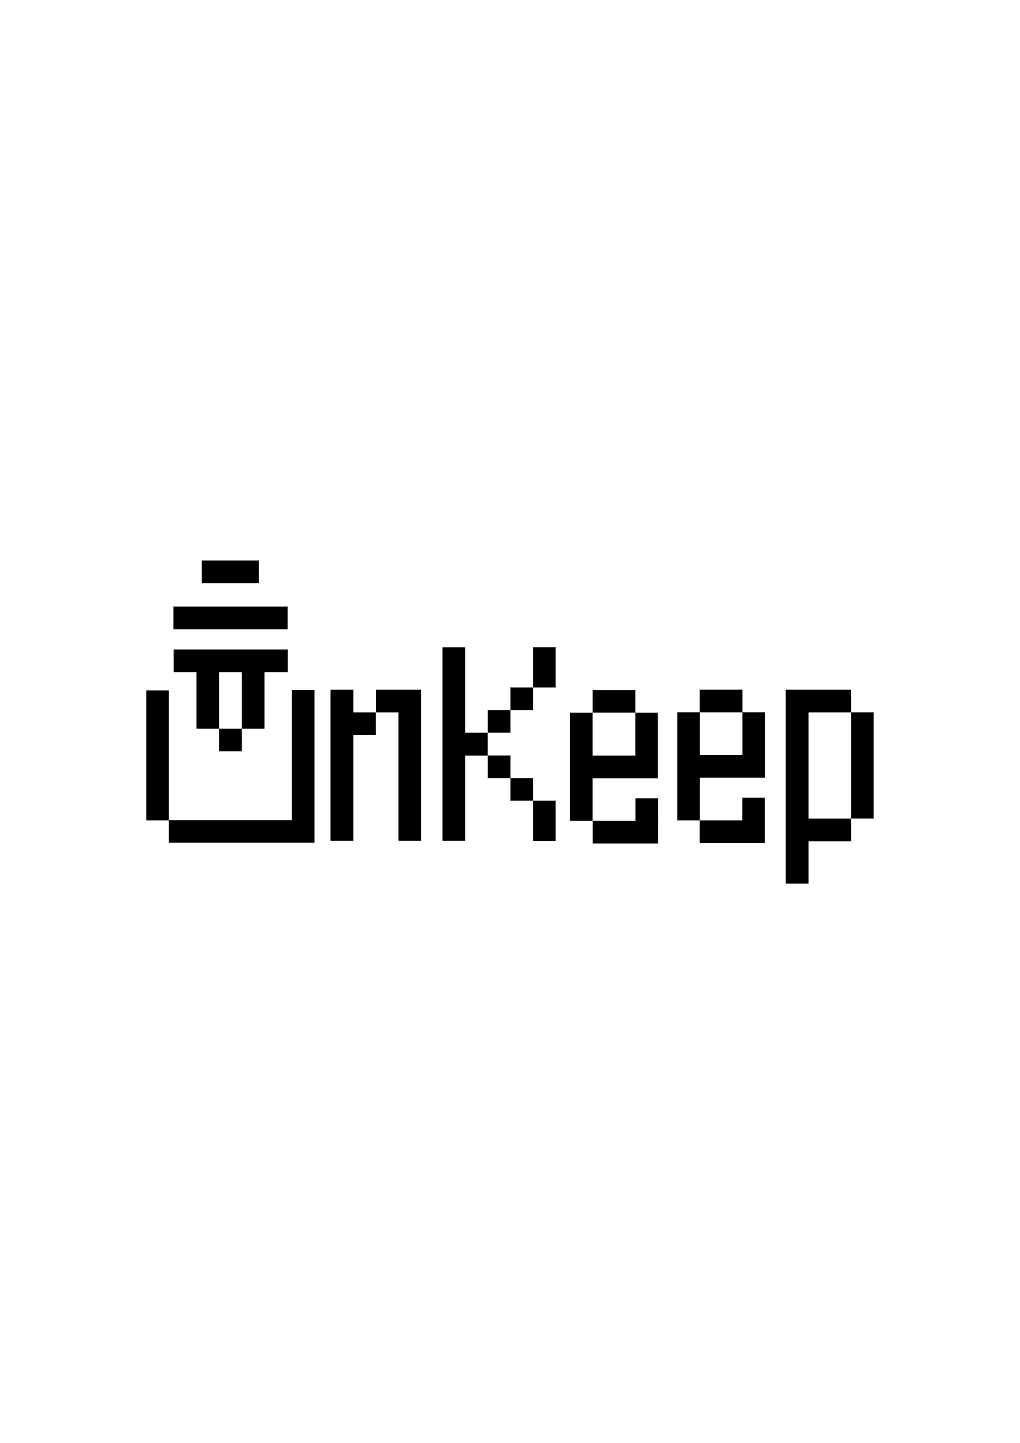
\includegraphics[width=0.5\textwidth]{./Resources/unKeepLogo.png}
            \end{figure}
       \vspace{0.5cm}

       \textbf{Alessandro Luppino}

       \vfill
            
       Politecnico di Bari\\
       Fondamenti del Web
            
       \vspace{0.1cm}
   \end{center}
\end{titlepage}
\tableofcontents
\newpage
\section{Introduzione}
unKeep è una web application per la gestione e condivisione di note. Estende il concetto tradizionale di note-taking con funzionalità di collaborazione in tempo reale e un sistema di versioning che permette di visualizzare, ripristinare e gestire le versioni precedenti delle note.
Il progetto è completamente hostato e accessibile all'indirizzo \url{https://unkeep.onrender.com}. Per scopi di sviluppo e testing locale, viene fornito un file \texttt{docker-compose.yml} che permette il deploy dell'intera applicazione \texttt{[Frontend :8080, Backend :8000, Database :27018]} in ambiente di sviluppo.
\section{Architettura del'applicazione}
\subsection{Autenticazione}
Al primo accesso al sito, l’utente viene reindirizzato alla pagina di login, qui può scegliere se effettuare il login o registrarsi. \\
La procedura di registrazione richiede l’inserimento di un username, di una password e di un indirizzo email. I dati vengono inviati al backend, che verifica la conformità ai requisiti del modello di dati. La password viene sottoposta ad hashing e, in caso di esito positivo, viene creato un nuovo utente nel database. Al termine, l’utente viene autenticato automaticamente. \\
La procedura di login prevede invece l’inserimento di username (o email) e password. Le credenziali fornite vengono confrontate con quelle presenti nel database; in caso di corrispondenza l’autenticazione ha successo e l’utente viene reindirizzato alla dashboard.\\
Una volta autenticato, all’utente vengono forniti due token JWT (JSON Web Token): un \textit{access token} con breve durata (15 minuti) e un \textit{refresh token} con durata più lunga (7 giorni). L’access token autentica le richieste al backend, mentre il refresh token consente di ottenere un nuovo access token quando quello corrente scade. \\
Il refreshToken viene memorizzato in cookie \texttt{HttpOnly} per migliorare la sicurezza contro attacchi XSS. In caso di scadenza dell’access token, il frontend invia automaticamente una richiesta al backend per ottenere un nuovo token utilizzando il refresh token. Se anche il refresh token è scaduto, l’utente viene disconnesso tramite logout e reindirizzato alla pagina di login. \\
La procedura di logout prevede la cancellazione dei cookie contenenti i token e la terminazione della sessione utente e potrà essere utilizzata anche dall'utente tramite la navbar che si trova in dashboard.
\begin{figure}[H]
    \centering
    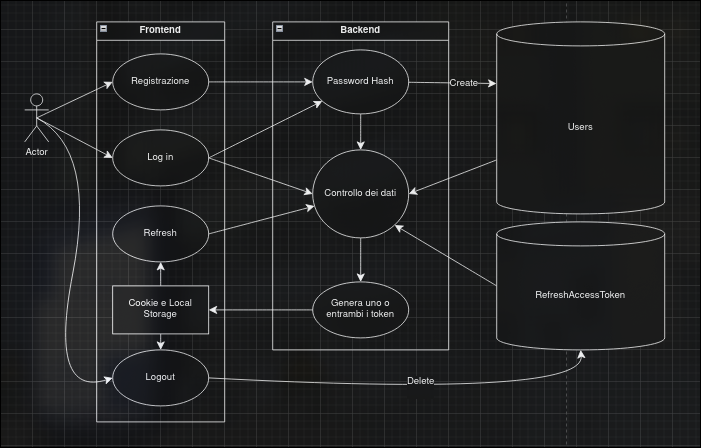
\includegraphics[width=0.65\textwidth]{./Resources/Diagrams/UML-Autenticazione.png}
\end{figure}
\subsection{Dashboard}
Dopo l’autenticazione, l’utente viene reindirizzato alla dashboard. \\
La dashboard presenta una \textit{navbar} che consente di accedere al proprio profilo. \\
Nella sezione principale viene mostrato l’elenco delle note: sia quelle create dall’utente, sia quelle condivise con lui da altri utenti. Per ciascuna nota vengono visualizzate informazioni sintetiche come l’autore, i collaboratori con permessi di scrittura, le eventuali tag e la data dell’ultima modifica. Inoltre è possibile creare una nuova nota. \\
\begin{figure}[H]
    \centering
    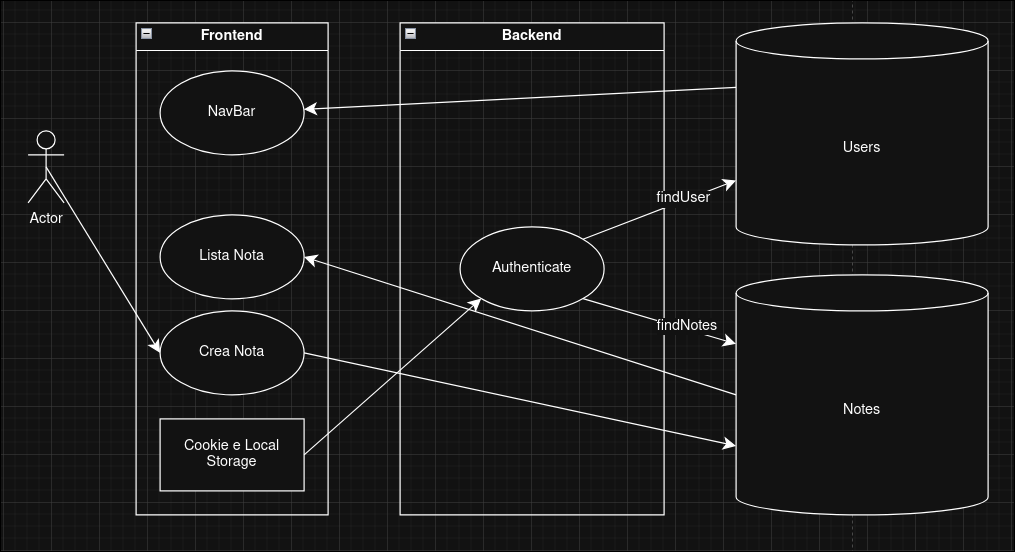
\includegraphics[width=0.5\textwidth]{./Resources/Diagrams/UML-Dashboard.png}
\end{figure}
\subsection{Gestione utente}
In questa sezione l’utente può visualizzare e modificare le informazioni del proprio profilo, come username, email e password. \\
È inoltre possibile aggiornare l’immagine del profilo, caricando una nuova immagine che viene salvata su \textit{Cloudinary}, mentre il relativo link viene memorizzato nel database. \\
Infine, l’utente ha la possibilità di eliminare definitivamente il proprio account. Tale operazione comporta la cancellazione di tutte le note create e la rimozione dell’utente dal database. In alternativa, l’utente può scegliere di migrare le proprie note al primo collaboratore associato a ciascuna di esse, qualora presente. In ogni caso la cronologia delle note verrà eliminata.
\begin{figure}[H]
    \centering
    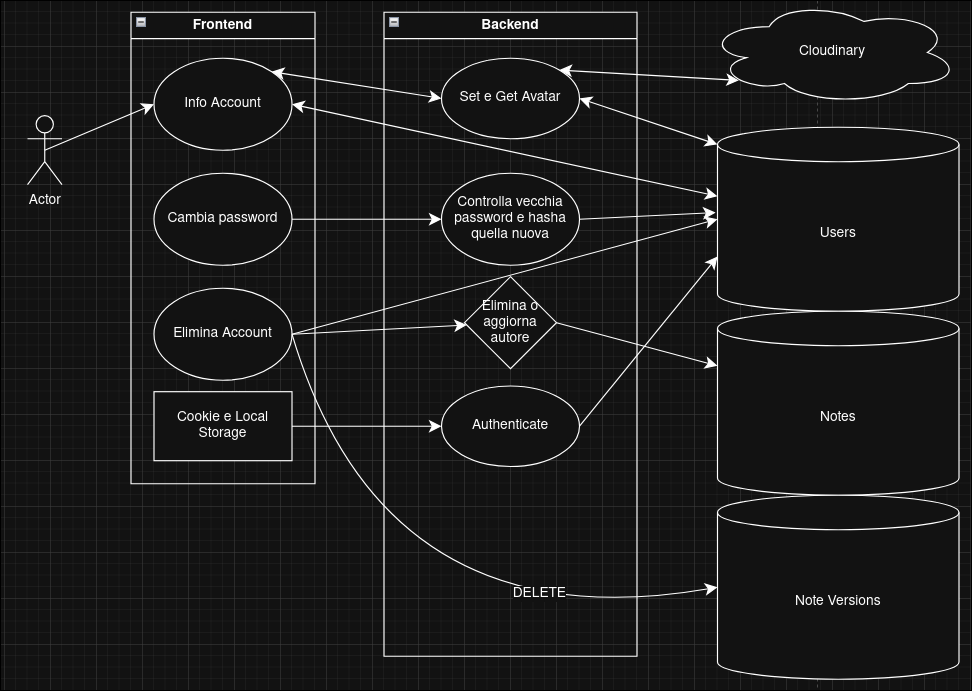
\includegraphics[width=0.7\textwidth]{./Resources/Diagrams/UML-Account.png}
\end{figure}
\subsection{Nota}
L’utente accede all'editor della nota selezionandola dalla dashboard oppure creando una nuova nota. \\
In base ai permessi assegnati, l’utente può assumere uno dei seguenti ruoli rispetto alla nota:
\begin{itemize}
    \item \textbf{Autore:} ha creato la nota. Può modificare il contenuto e il titolo, salvare i cambiamenti ed accedere al pannello di gestione avanzata della nota.
    \item \textbf{Collaboratore con permessi di scrittura:} può modificare esclusivamente il contenuto della nota e salvarne le modifiche.
    \item \textbf{Collaboratore con permessi di sola lettura:} può visualizzare il contenuto della nota, senza possibilità di modificarlo o salvarlo.
\end{itemize}
L’editor di testo è implementato con \textit{Quill}, che consente la modifica collaborativa e la visualizzazione dei cursori degli altri utenti in tempo reale grazie all’estensione \textit{Quill Cursors}. \\
La sincronizzazione in tempo reale è gestita tramite \textit{Socket.IO}, che permette di propagare le modifiche a tutti i collaboratori connessi. Gli utenti dotati di permessi adeguati possono salvare le modifiche apportate, generando una nuova versione e aggiornando contestualmente quella corrente.
\begin{figure}[H]
    \centering
    \begin{minipage}[t]{0.23\textwidth}
        \vspace{0pt}
        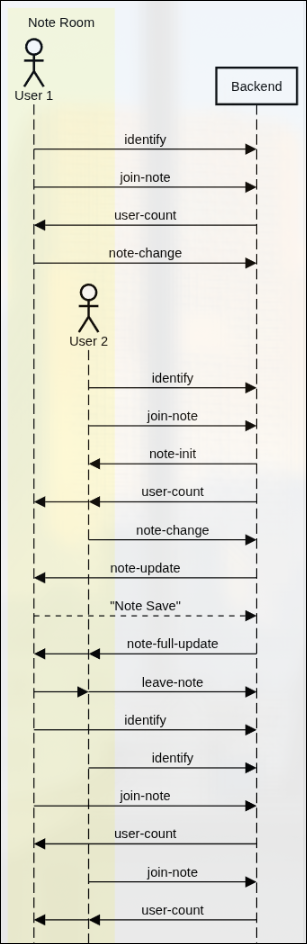
\includegraphics[width=\linewidth]{./Resources/Diagrams/UML-NotaSequenze.png}
    \end{minipage}
    \begin{minipage}[t]{0.75\textwidth}
        \vspace{0pt}
        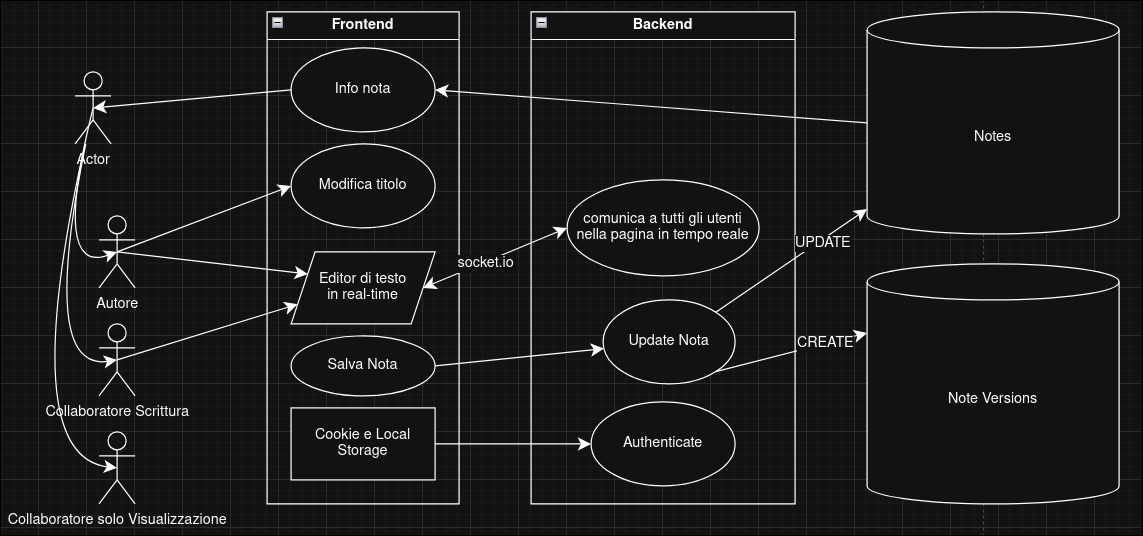
\includegraphics[width=\linewidth]{./Resources/Diagrams/UML-Nota.png}
    \end{minipage}\hfill
\end{figure}
\newpage
\subsection{Gestione della nota}
La gestione della nota è disponibile esclusivamente per l’autore e comprende le seguenti funzionalità: \\
\textbf{Cronologia versioni (in tempo reale):}
\begin{itemize}
    \item Visualizzazione delle versioni salvate, con indicazione di autore e timestamp.
    \item Ripristino della nota a una versione precedente (\textit{revert}).
    \item Eliminazione delle versioni antecedenti a quella selezionata (\textit{rebase}).
\end{itemize}
\textbf{Gestione collaboratori:}
\begin{itemize}
    \item Aggiunta collaboratori tramite ricerca per \textit{username}.
    \item Rimozione collaboratori.
    \item Modifica permessi (scrittura/sola lettura).
\end{itemize}
\textbf{Gestione tag:}
\begin{itemize}
    \item Aggiunta e rimozione di tag associate alla nota.
\end{itemize}
Oltre alla possibilità di eliminare o salvare la nota.\\ 
Quando una nota viene salvata i cambiamenti vengono inviati ai collaboratori nell'editor in tempo reale.
\begin{figure}[H]
    \centering
    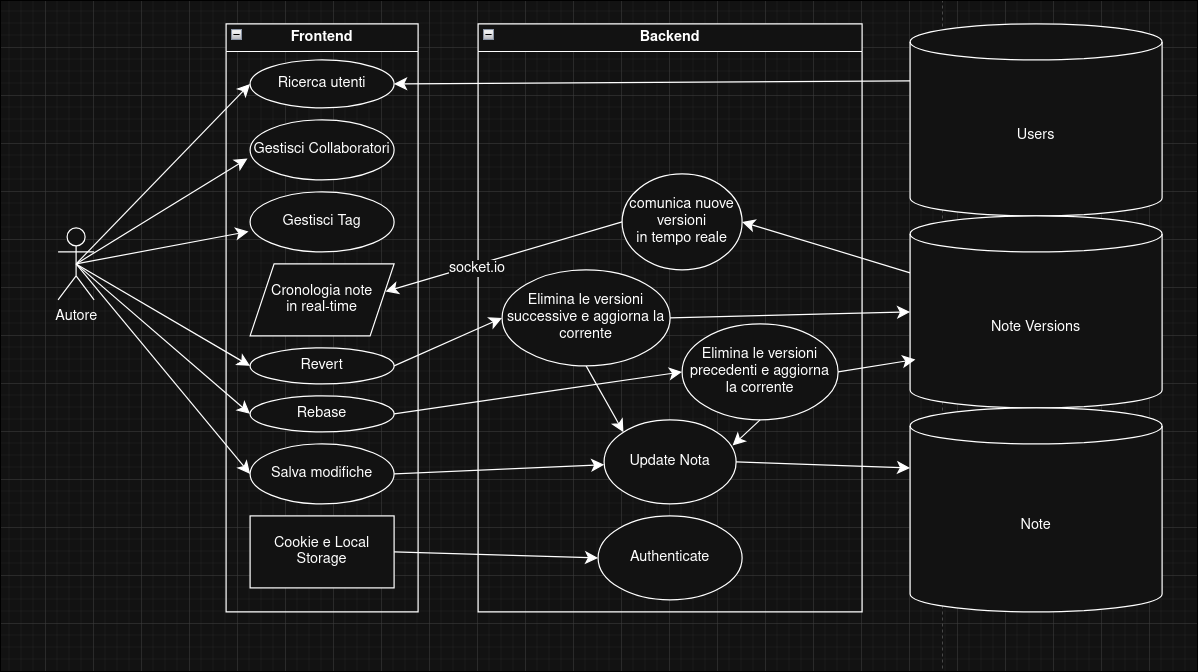
\includegraphics[width=1\textwidth]{./Resources/Diagrams/UML-ImpostazioniNota.png}
\end{figure}

\newpage

\section{Modello dei dati}

\subsection{User}
Lo schema \texttt{User} rappresenta gli utenti registrati nell’applicazione.  
\begin{itemize}
    \item \textbf{username} (\texttt{String}, obbligatorio, unico): deve contenere da 3 a 20 caratteri alfanumerici. 
    \item \textbf{email} (\texttt{String}, obbligatorio, unico): validata tramite espressione regolare, salvata in minuscolo.
    \item \textbf{password} (\texttt{String}, obbligatorio): da 6 a 128 caratteri, deve contenere almeno una lettera maiuscola, un numero e un carattere speciale.
    \item \textbf{avatar} (\texttt{String}, opzionale): URL dell’immagine profilo, di default stringa vuota.
    \item \textbf{createdAt} (\texttt{Date}): data di creazione dell’account, impostata automaticamente.
\end{itemize}

\subsection{Note}
Lo schema \texttt{Note} rappresenta le note create dagli utenti.  
\begin{itemize}
    \item \textbf{title} (\texttt{String}, obbligatorio): da 1 a 50 caratteri, gli spazi in eccesso vengono rimossi.
    \item \textbf{content} (\texttt{String}, opzionale): contenuto della nota, fino a 100000 caratteri.
    \item \textbf{author} (\texttt{ObjectId}, obbligatorio): riferimento all’utente autore della nota.
    \item \textbf{collaborators} (\texttt{Array}):
        \begin{itemize}
            \item \textbf{user} (\texttt{ObjectId}, obbligatorio): riferimento a un utente collaboratore.
            \item \textbf{permission} (\texttt{String}, obbligatorio): permessi assegnati, valori ammessi: \texttt{read}, \texttt{write}.
        \end{itemize}
    \item \textbf{tags} (\texttt{Array di String}): tag testuali (max 30 caratteri) per organizzare le note.
    \item \textbf{currentVersion} (\texttt{Number}): versione corrente della nota, aggiornata automaticamente.
    \item \textbf{timestamps}: campi automatici \texttt{createdAt} e \texttt{updatedAt}.
\end{itemize}

\subsection{NoteVersion}
Lo schema \texttt{NoteVersion} gestisce la cronologia delle versioni delle note.  
\begin{itemize}
    \item \textbf{noteId} (\texttt{ObjectId}, obbligatorio): riferimento alla nota associata.
    \item \textbf{createdBy} (\texttt{ObjectId}, obbligatorio): riferimento all’utente che ha creato la versione.
    \item \textbf{delta} (\texttt{Array di Mixed}): insieme delle modifiche (diff) rispetto alla versione precedente.
    \item \textbf{baseVersion} (\texttt{Number}, obbligatorio): numero della versione di riferimento.
    \item \textbf{createdAt} (\texttt{Date}): data di creazione della versione, impostata automaticamente.
\end{itemize}

\subsection{RefreshToken}
Lo schema \texttt{RefreshToken} gestisce i token di refresh degli utenti.  
\begin{itemize}
    \item \textbf{userId} (\texttt{ObjectId}, obbligatorio): riferimento all’utente proprietario del token.
    \item \textbf{token} (\texttt{String}, obbligatorio): valore del token JWT.
    \item \textbf{createdAt} (\texttt{Date}): data di creazione, impostata automaticamente. Il campo include un TTL di 14 giorni, dopo i quali il documento viene eliminato automaticamente dal database.
\end{itemize}
\newpage
% DOCUMENTAZIONE
\section{Documentazione API}
Ogni endpoint restituisce risposte in formato JSON con messaggi di successo o errore. Non verranno documentati, ma si farà riferimento ai codici di stato HTTP standard per indicare il risultato delle operazioni.
\subsection{Autenticazione e Autorizzazione (Auth)}
\subsubsection{\texttt{POST /auth/register}}
\begin{itemize}
    \item \textbf{Descrizione}: Registra un nuovo utente nel sistema.
    \item \textbf{Metodo}: \texttt{POST}.
    \item \textbf{Autenticazione}: Nessuna (endpoint pubblico).
    \item \textbf{Body (raw JSON)}: Richiede un oggetto JSON contenente l'\texttt{username}, l'\texttt{email} e la \texttt{password} del nuovo utente.
\end{itemize}

\subsubsection{\texttt{POST /auth/login}}
\begin{itemize}
    \item \textbf{Descrizione}: Autentica un utente e restituisce un \texttt{accessToken} come json e un \texttt{refreshToken} come cookie \texttt{HttpOnly}.
    \item \textbf{Autenticazione}: Nessuna (endpoint pubblico).
    \item \textbf{Body (raw JSON)}: Richiede un oggetto JSON contenente l'email o l'username in \texttt{emailOrUsername} e la \texttt{password} dell'utente.
\end{itemize}

\subsubsection{\texttt{POST /auth/refresh}}
\begin{itemize}
    \item \textbf{Descrizione}: Aggiorna l'\texttt{accessToken} utilizzando il \texttt{refreshToken} fornito nel cookie \texttt{HttpOnly}.
    \item \textbf{Metodo}: \texttt{POST}.
    \item \textbf{Autenticazione}: Nessuna (endpoint pubblico).
\end{itemize}

\subsubsection{\texttt{POST /auth/logout}}
\begin{itemize}
    \item \textbf{Descrizione}: Disconnette l'utente corrente eliminando il \texttt{refreshToken} dal database e cancellando il cookie.
    \item \textbf{Metodo}: \texttt{POST}.
    \item \textbf{Autenticazione}: Richiede \texttt{Bearer Token}.
\end{itemize}

\subsubsection{\texttt{POST /auth/change-password}}
\begin{itemize}
    \item \textbf{Descrizione}: Permette all'utente autenticato di cambiare la propria password.
    \item \textbf{Metodo}: \texttt{POST}.
    \item \textbf{Autenticazione}: Richiede \texttt{Bearer Token}.
    \item \textbf{Body (raw JSON)}: Richiede un oggetto JSON contenente la \texttt{currentPassword} e la \texttt{newPassword}.
\end{itemize}

\subsection{Gestione Note (Notes)}
\subsubsection{\texttt{POST /notes}}
\begin{itemize}
    \item \textbf{Descrizione}: Crea una nuova nota.
    \item \textbf{Metodo}: \texttt{POST}.
    \item \textbf{Autenticazione}: Richiede \texttt{Bearer Token}.
    \item \textbf{Body (raw JSON)}: Richiede un oggetto JSON con il \texttt{title} della nota e opzionalmente: il \texttt{content}, un array di \texttt{collaborators} (ciascuno con un \texttt{user} ID e un \texttt{permission}), e un array di \texttt{tags}.
\end{itemize}

\subsubsection{\texttt{GET /notes}}
\begin{itemize}
    \item \textbf{Descrizione}: Recupera tutte le note di cui l’utente autenticato è autore o collaboratore. 
    Le note senza cronologia associata vengono considerate temporanee e non vengono restituite; 
    durante la chiamata esse vengono rimosse dal database per garantire coerenza dei dati.
    \item \textbf{Metodo}: \texttt{GET}.
    \item \textbf{Autenticazione}: Richiede \texttt{Bearer Token}.
\end{itemize}

\subsubsection{\texttt{GET /notes/\{noteId\}}}
\begin{itemize}
    \item \textbf{Descrizione}: Recupera una specifica nota tramite il suo ID se l'utente autenticato è l'autore o un collaboratore.
    \item \textbf{Metodo}: \texttt{GET}.
    \item \textbf{Autenticazione}: Richiede \texttt{Bearer Token}.
    \item \textbf{Parametri Path}: il \texttt{\{noteId\}} della nota da recuperare [\texttt{String}].
\end{itemize}

\subsubsection{\texttt{PUT /notes/\{noteId\}}}
\begin{itemize}
    \item \textbf{Descrizione}: Aggiorna una nota esistente tramite il suo ID se l'utente autenticato è l'autore può modificare tutti i campi, mentre i collaboratori con permessi di scrittura possono modificare solo il \texttt{content}. Se la nota non ha cronologia viene creata la prima versione, altrimenti viene creata una nuova versione con le modifiche.
    \item \textbf{Metodo}: \texttt{PUT}.
    \item \textbf{Autenticazione}: Richiede \texttt{Bearer Token}.
    \item \textbf{Parametri Path}: il \texttt{\{noteId\}} della nota da aggiornare [\texttt{String}].
    \item \textbf{Body (raw JSON)}: Richiede un oggetto JSON contenente almeno uno di questi campi \texttt{title}, \texttt{content}, array di \texttt{collaborators} (ciascuno con un \texttt{user} ID e un \texttt{permission}) o un array di \texttt{tags} diversi da quelli attuali.
\end{itemize}

\subsubsection{\texttt{DELETE /notes/\{noteId\}}}
\begin{itemize}
    \item \textbf{Descrizione}: Elimina una nota e tutte le sue versioni tramite il suo ID.
    \item \textbf{Metodo}: \texttt{DELETE}.
    \item \textbf{Autenticazione}: Richiede \texttt{Bearer Token}.
    \item \textbf{Parametri Path}: il \texttt{\{noteId\}} della nota da eliminare [\texttt{String}].
\end{itemize}

\subsection{Cronologia Note (Versions)}
Accessibili solo dall'autore della nota.
\subsubsection{\texttt{GET /notes/\{noteId\}/versions?type=\{string\}}}
\begin{itemize}
    \item \textbf{Descrizione}: Recupera la cronologia delle versioni per una specifica nota tramite il suo ID.
    \item \textbf{Metodo}: \texttt{GET}.
    \item \textbf{Autenticazione}: Richiede \texttt{Bearer Token}.
    \item \textbf{Parametri Path}: il \texttt{\{noteId\}} della nota [\texttt{String}].
    \item \textbf{Parametri Query}: \texttt{type=\{"delta"\}} opzionale, default: "delta". Attualmente è l'unico valore supportato.
\end{itemize}

\subsubsection{\texttt{GET /notes/\{noteId\}/versions/\{version\}?type=\{string\}}}
\begin{itemize}
    \item \textbf{Descrizione}: Recupera una specifica versione di una nota tramite il suo ID e il numero di versione.
    \item \textbf{Metodo}: \texttt{GET}.
    \item \textbf{Autenticazione}: Richiede \texttt{Bearer Token}.
    \item \textbf{Parametri Path}: il \texttt{\{noteId\}} della nota [\texttt{String}] e il numero di \texttt{\{version\}} da recuperare [\texttt{Int}].
    \item \textbf{Parametri Query}: \texttt{type=\{"delta", "full"\}} opzionale, default: "delta".  "delta" restituisce solo le modifiche rispetto alla versione precedente, mentre "full" restituisce il contenuto completo della nota a quella versione.
\end{itemize}

\subsubsection{\texttt{POST /notes/\{noteId\}/versions/\{version\}/revert}}
\begin{itemize}
    \item \textbf{Descrizione}: Ripristina una nota alla versione precedente specificata ed elimina tutte le versioni successive.
    \item \textbf{Metodo}: \texttt{POST}.
    \item \textbf{Autenticazione}: Richiede \texttt{Bearer Token}.
    \item \textbf{Parametri Path}: il \texttt{\{noteId\}} della nota [\texttt{String}] e il numero di \texttt{\{version\}} a cui ripristinare [\texttt{Int}].
\end{itemize}

\subsubsection{\texttt{POST /notes/\{noteId\}/versions/\{version\}/rebase}}
\begin{itemize}
    \item \textbf{Descrizione}: Sposta la versione "0" della nota alla versione specificata, eliminando tutte le versioni precedenti. Non modifica la versione corrente della nota.
    \item \textbf{Metodo}: \texttt{POST}.
    \item \textbf{Autenticazione}: Richiede \texttt{Bearer Token}.
    \item \textbf{Parametri Path}: il \texttt{\{noteId\}} della nota [\texttt{String}] e il numero di \texttt{\{version\}} a cui effettuare il rebase [\texttt{Int}].
\end{itemize}

\subsection{Gestione Utenti (Users)}

\subsubsection{\texttt{GET /users?q=\{string\}}}
\begin{itemize}
    \item \textbf{Descrizione}: Ricerca utenti per username utilizzando una stringa di query.
    \item \textbf{Metodo}: \texttt{GET}.
    \item \textbf{Autenticazione}: Richiede \texttt{Bearer Token}.
    \item \textbf{Parametri Query}: \texttt{q=\{query\}}, obbligatorio. Rappresenta la stringa di ricerca deve essere almeno di 2 caratteri.
\end{itemize}

\subsubsection{\texttt{GET /users/me}}
\begin{itemize}
    \item \textbf{Descrizione}: Recupera il profilo dell'utente autenticato. Se viene fornito un file 
    \item \textbf{Metodo}: \texttt{GET}.
    \item \textbf{Autenticazione}: Richiede \texttt{Bearer Token}.
\end{itemize}

\subsubsection{\texttt{PUT /users/me}}
\begin{itemize}
    \item \textbf{Descrizione}: Aggiorna le informazioni del profilo dell’utente autenticato (username, email e avatar). 
    Supporta la sostituzione o la rimozione dell’avatar, gestendo l’upload su \textit{Cloudinary} e l’eventuale eliminazione dell’immagine precedente. 
    Restituisce un errore se non viene effettuata alcuna modifica.
    \item \textbf{Metodo}: \texttt{PUT}.
    \item \textbf{Autenticazione}: Richiede \texttt{Bearer Token}.
    \item \textbf{Body (JSON o multipart/form-data)}: \texttt Richiede un \texttt{username} una \texttt{email} e opzionalmente un \texttt{avatar} che può essere un file o una stringa.
\end{itemize}

\subsubsection{\texttt{DELETE /users?migrateNotes=\{boolean\}}}
\begin{itemize}
    \item \textbf{Descrizione}: Elimina l’account dell’utente autenticato. 
    Se il parametro \texttt{migrateNotes} è impostato, le note create dall’utente vengono migrate al primo collaboratore con permessi di scrittura, altrimenti tutte le note e le relative versioni vengono eliminate. 
    L’utente viene inoltre rimosso come collaboratore dalle note di altri utenti, e il refresh token viene invalidato.
    \item \textbf{Metodo}: \texttt{DELETE}.
    \item \textbf{Autenticazione}: Richiede \texttt{Bearer Token}.
    \item \textbf{Parametri Query}: \texttt{migrateNotes}, opzionale. Se presente, attiva la migrazione delle note al primo collaboratore disponibile.
\end{itemize}

\newpage
\section{Componenti React}

\paragraph{App}  
Componente principale dell’applicazione. Inizializza la connessione WebSocket con il backend (\texttt{socket.io-client}). Applica il tema globale tramite \texttt{CustomThemeProvider}.  Gestisce il routing con \texttt{BrowserRouter}.  Fornisce contesto di autenticazione (\texttt{AuthProvider}).  Carica le rotte definite in \texttt{AppRoutes}.

\paragraph{Main}
Componente che racchiude la struttura principale dell’applicazione.

\paragraph{AppRoutes}  
Gestore centrale delle rotte. Definisce tutte le rotte principali con \texttt{react-router}. Utilizza \texttt{ProtectedRoute} per le pagine accessibili solo ad utenti autenticati (\texttt{Dashboard}, \texttt{MyProfile}, \texttt{ChangePassword}, \texttt{NoteEdit}, \texttt{NoteSettings}). Gestisce rotta “catch-all” (\texttt{*}) mostrando \texttt{Navbar} ed \texttt{ErrorBanner 404}.

\subsection{Components}

\paragraph{AddNoteFab} 
Pulsante flottante per la creazione di una nuova nota. 
È sempre visibile in basso a destra della dashboard.

\paragraph{AvatarField} 
Campo che permette di caricare, visualizzare e rimuovere un avatar utente. 
Mostra l’avatar corrente tramite \texttt{CustomAvatar}, con la possibilità di selezionare una nuova immagine da file locale o rimuoverla tramite un pulsante di chiusura. 
Gestisce interazioni utente legate all’immagine del profilo.

\paragraph{CustomAvatar} 
\texttt{Avatar} di MUI personalizzato per la visualizzazione di un avatar che utilizzi il logo dell’applicazione come contenuto se non viene fornita un’immagine.
Il colore di sfondo è generato dinamicamente dalla funzione \texttt{stringToColor}, che trasforma una stringa (tipicamente lo username) in un colore HSL stabile e unico.  
La funzione è esportata separatemente e viene utilizzata anche in altri componenti garantendo coerenza cromatica tra gli utenti.

\paragraph{DashboardBanner} 
Banner informativo per la dashboard. 
Mostra opzionalmente un titolo e un messaggio, centrati all’interno di una card. 
Supporta contenuti aggiuntivi tramite \texttt{children}, per includere pulsanti o altri elementi UI a supporto del messaggio principale. Viene utilizzato per invitare a creare la prima nota quando l’elenco è vuoto.

\paragraph{DeleteDialog}  
Dialogo di conferma per la cancellazione di un’entità.  
Mostra titolo, descrizione, eventuali contenuti extra e un campo di input per confermare l’operazione (ad esempio digitando il nome della risorsa).  
Il pulsante di eliminazione è disabilitato finché il valore inserito non corrisponde a quello richiesto.  

\paragraph{ErrorBanner}  
Banner che visualizza un messaggio di errore per la dashboard.  
Mostra informazioni provenienti dall’oggetto \texttt{error}, come codice di stato HTTP, codice generico o messaggio.

\paragraph{ErrorLog}  
Lista animata capace di gestire più errori.  
Utilizza \texttt{Collapse} e \texttt{Transition Group} per mostrare e rimuovere dinamicamente gli errori. 

\paragraph{FormField}  
Campo di input con etichetta.  
Supporta sia input testuali standard che campi di tipo password (attraverso l’uso del componente \texttt{PasswordField}).

\paragraph{FormWrapper}  
Contenitore per form centrati nella pagina.  
Visualizza un titolo, un logo opzionale e un pulsante di chiusura in alto a destra.  
Gli elementi figli (\texttt{children}) rappresentano i campi o le azioni del form.

\paragraph{Logo}  
\texttt{Box} svg che mostra il logo dell’applicazione, si può personalizzare dimensione, colore e scegliere tra tre varianti: logotipo, logo e solo testo.

\paragraph{Navbar}  
Barra di navigazione superiore della dashboard. Cliccare il logo consente di ricaricare le note. Se l’utente non è autenticato: mostra pulsanti \texttt{Login} e \texttt{Sign Up}.  
Se autenticato: mostra nome utente, avatar personalizzato e un \texttt{Popover} a comparsa per navigare verso \texttt{Profile} oppure fare \texttt{Logout}.

\paragraph{Note}  
Card che rappresenta una singola nota. Mostra autore e collaboratori con permesso di scrittura con avatar cliccabili per visualizzare meglio l'avatar; titolo, contenuto, tag e data ultima modifica della nota. Se l’utente è autore mostra un pulsante per accedere alle impostazioni della nota.  
Cliccando sul contenuto si naviga all'edit della nota.

\paragraph{NoteList}  
Contenitore che gestisce l’elenco delle note. In fase di caricamento mostra placeholder con \texttt{Skeleton}.

\paragraph{NoteTitleBar}  
Componente che mostra il titolo della nota e permette di modificarla in base ai permessi dell'utente.  

\paragraph{PasswordField}  
Campo di input per password con possibilità di toggle della visibilità.

\paragraph{ProtectedRoute}
Componente che protegge le rotte che richiedono autenticazione reindirizzando alla pagina di login se l’utente non è autenticato.

\paragraph{UnsavedDialog}
Dialogo che avvisa quando l'ultimo utente presente nella nota tenta di navigare via da una nota con modifiche non salvate. 
Offre la possibilità di rimanere sulla pagina o procedere con la navigazione salvando oppure scartando le modifiche.

\paragraph{UserModal}
Modale che permette di visualizzare in grande l'avatar di un utente.

\paragraph{VersionModal}
Modale che permette di visualizzare una nota in una versione specifica.

\subsubsection{NoteSettingsTabs}
In questa cartella sono presenti i componenti che verranno renderizzati da NoteSettings
\paragraph{CollaboratorsTab} 
Scheda che permette di gestire i collaboratori di una nota. Permette di cercare utenti tramite username, aggiungerli come collaboratori con permessi iniziali di sola lettura, e visualizzare la lista dei collaboratori già presenti. 
L’autore della nota può modificare i permessi (lettura/scrittura) o rimuovere un collaboratore.

\paragraph{NoteHistoryTab} 
Scheda che mostra la cronologia delle versioni di una nota utilizzando una \texttt{Timeline} di Material UI. 
Ogni elemento della cronologia riporta l’autore della modifica, la data e l’ora di creazione, e consente di selezionare una versione per il revert o la visualizzazione. 
Il colore della versione è determinato dall’utente che ha effettuato la modifica.

\paragraph{TagsTab} 
Scheda che consente di aggiungere, visualizzare e rimuovere tag associati a una nota. 
I tag possono essere inseriti tramite un campo di input e non possono superare i 30 caratteri. 
Ogni tag viene rappresentato come una \texttt{Chip} interattiva che può essere eliminata con un’azione diretta dell’utente.

\subsection{Context}
\paragraph{AuthContext \& AuthProvider}  
Contesto globale per la gestione dell’autenticazione e delle operazioni con l’API backend.  
Fornisce metodi per:  
\begin{itemize}
  \item Registrazione, login, logout e refresh del token di accesso.  
  \item Gestione profilo utente (lettura, aggiornamento, cambio password, eliminazione con opzione di migrazione note).  
  \item Operazioni sulle note (creazione, modifica, eliminazione, recupero) e sulle versioni delle note (cronologia, revert, rebase).  
  \item Ricerca di altri utenti.  
\end{itemize}
Integra un \texttt{axios interceptor} per il refresh automatico dei token scaduti.  
\texttt{useAuth()} è l’hook che permette l’accesso ai metodi e allo stato del contesto. 

\subsection{Hooks}
\paragraph{useControlledNavigation}  
Hook personalizzato che permette di intercettare e controllare la navigazione condizionata.  
\begin{itemize}
  \item Accetta un flag \texttt{shouldBlock} per bloccare temporaneamente la navigazione.  
  \item Fornisce una funzione di navigazione che, se bloccata, salva la destinazione in sospeso.  
  \item Espone metodi \texttt{confirm()} e \texttt{cancel()} per rispettivamente confermare o annullare la navigazione salvata.  
\end{itemize}

\subsection{Pages}
\paragraph{ChangePassword}  
Pagina che permette all’utente autenticato di cambiare la propria password.

\paragraph{Dashboard}  
Pagina principale dell’applicazione, accessibile solo ad utenti autenticati.

\paragraph{Login}  
Pagina di login per utenti esistenti.

\paragraph{MyProfile}  
Pagina di gestione del profilo utente, accessibile solo ad utenti autenticati.

\paragraph{NoteEdit}  
Pagina di modifica in tempo reale di una nota, accessibile solo ad utenti autenticati che sono autori o collaboratori della nota.

\paragraph{NoteSettings}
Pagina di gestione delle impostazioni di una nota, accessibile solo all’autore della nota.

\paragraph{SignUp}
Pagina di registrazione per nuovi utenti.

\subsection{Theme}
\paragraph{CustomThemeProvider}  
Tema MUI personalizzato all’applicazione.  
Le principali personalizzazioni includono:  
\begin{itemize}
  \item Palette colori (testo, primario, errori, sfondi).  
  \item Tipografia (font \texttt{Lexend} e \texttt{Tiny5} con pesi e dimensioni personalizzate).  
  \item Stili globali per componenti MUI (\texttt{Tooltip}, \texttt{Popover}, \texttt{Button}, \texttt{IconButton}, \texttt{FormLabel}, \texttt{DialogTitle}).  
\end{itemize}
Tutti i figli (\texttt{children}) sono resi all’interno del \texttt{ThemeProvider}.  

\end{document}